%!TEX root = ../my_thesis.tex
\chapter{Techniques for fast z feedback}

Several people have improved the AFM feedback loop by implementing model based controller or high frequency actuators. The drawback with these actuators is the decrease in the positioning range.
/CURRENT FEEDBACK SCHEME

We have decided to improve the bandwidth and the scan range of our device. 
Many people have improved the bandwidth of their AFM by designing a dual integrated actuators system \cite{sulchek1999dual}. Most of them have introduced an external piezoelectrical actuator on top of the cantilever. With this scheme, we can combine the advantages of a high bandwidth from the piezo-electrical actuator and the long range of the tip.

/PREVIOUS METHOD OF TILT




\section{Double PID}

The principal feature of an AFM is it's probing system. \cite{jeong:093706} The feedback control system is designed to adjust the motion of the tip on the z-axis. It will adjust the tip-to-sample distance. We have developed a dual-actuator control system. 

We put a piezo-electrical ceramics on top of the X-Y scanner. This device will work with the scanner to achieve a larger bandwidth. Indeed, it picks up high spatial frequency topography. 

\begin{figure}[H]
  \centering
  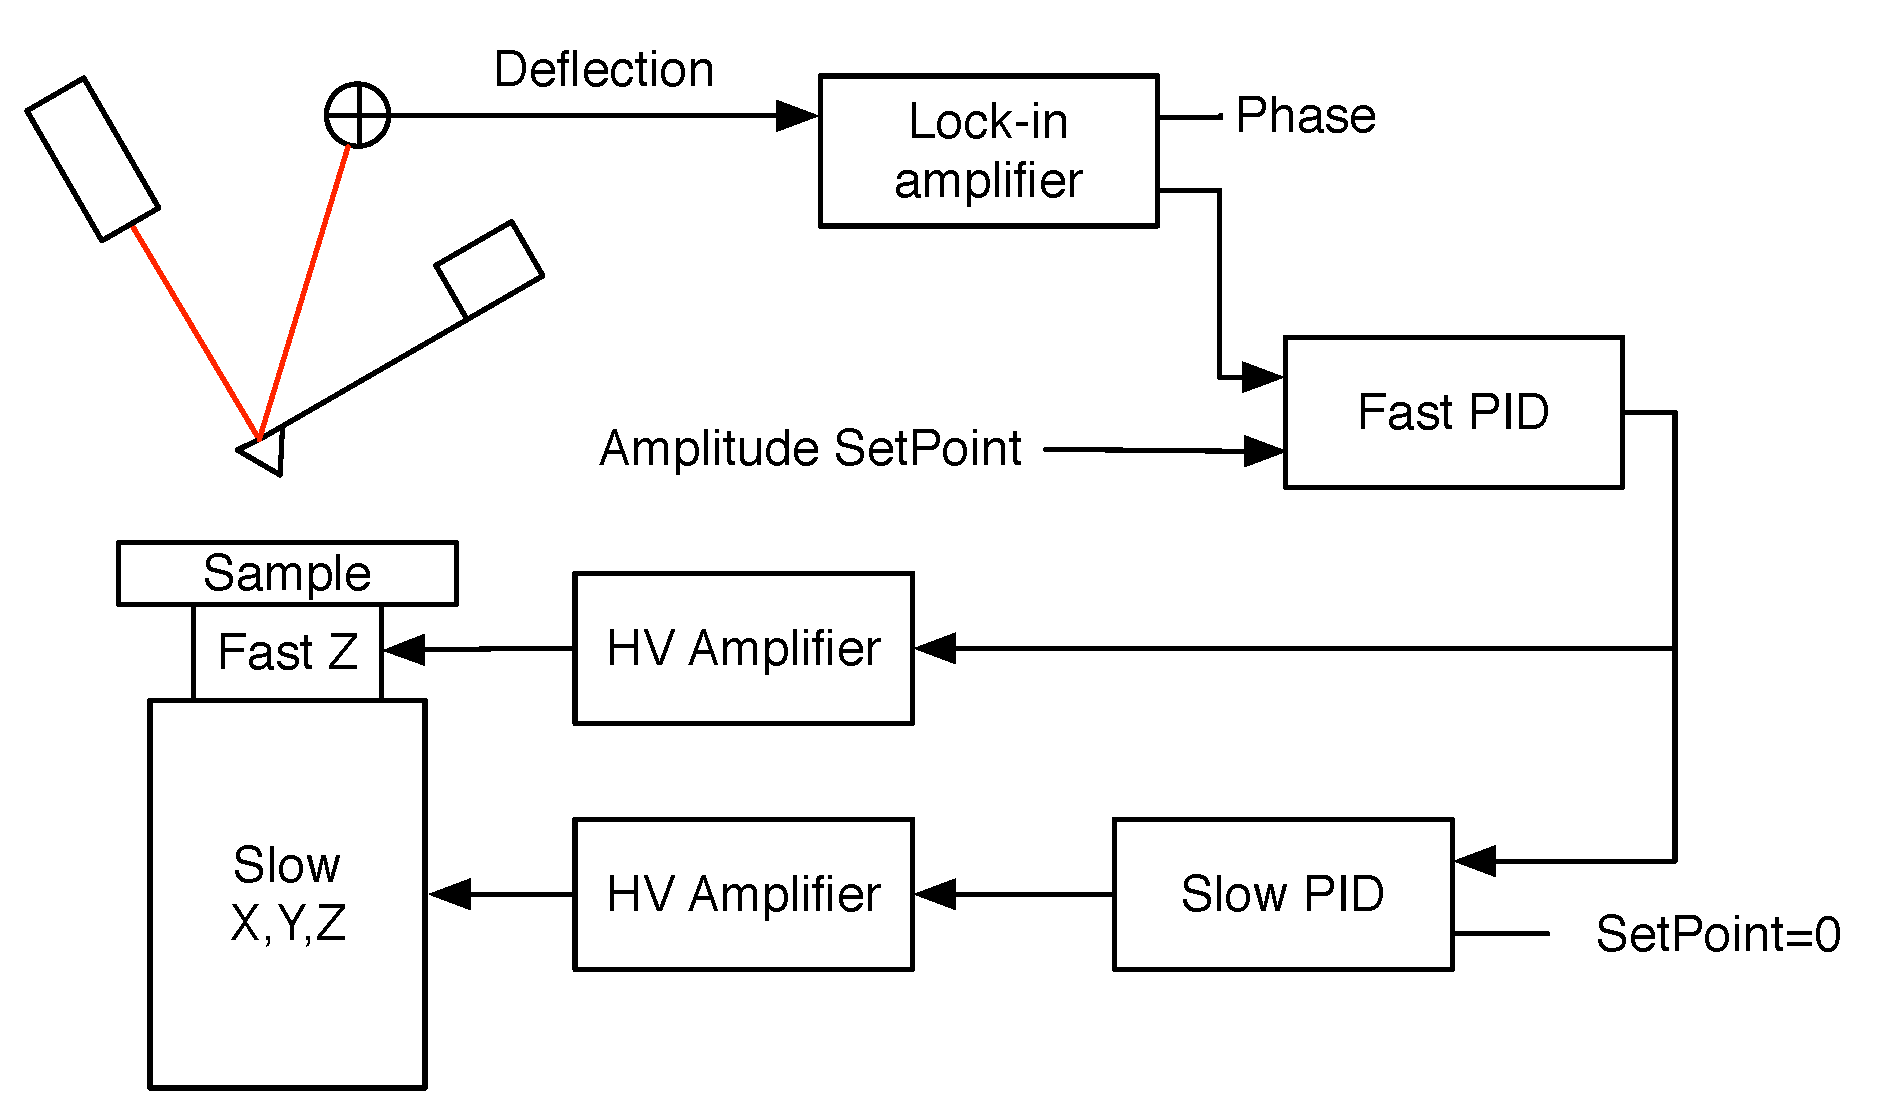
\includegraphics[scale=0.3]{images/doublePID.eps}
    \caption{Double PID}
  \label{DoublePid}
\end{figure}



\section{Tilt compensation}

If the probe/sample angle is not perpendicular, we observe a tilt on the surface. This tilt is problematic when it becomes larger than the features. Flattening algorithms restore the image and put the data on the same level. This technique works if the range of the tip is large enough. We have decided to take another approach and to dynamically compensate for the tilt.

First, we scan the surface of the sample with a circle pattern. It gives us informations about the general topography of the surface. Then, we compute the plane equation of the surface by applying a fit in Igor Pro.

\begin{equation}\label{eqn:planeeq}
z = a_1 x + a_2 y + a_3 
\end{equation}

We find the coefficients by minimizing the values of Chi-Square. Then, we generate the waves to send to the controller the following way.

\begin{equation}\label{eqn:sendwave}
wavetosend = a_1 wavex + a_2 wavey 
\end{equation}

\subsection{Experiment}

Wavex and wavey are the x,y components of our scan pattern. The scan pattern for an Archimedean spiral is defined by the equation  ~\ref{eqarchimedean}.

\begin{equation}\label{eqarchimedean}
x(t)= \alpha \sqrt{t} cos(\beta \sqrt{t})
y(t)= \alpha \sqrt{t} sin(\beta \sqrt{t})
\end{equation}

We took a calibration sample to test the efficiency of our method. The size or our scan is 30um. We see on the figure  ~\ref{tiltcircle} that the surface has a tilt. The small spikes on the curve represent the pyramids on the sample.


\begin{figure}[H]
  \centering
  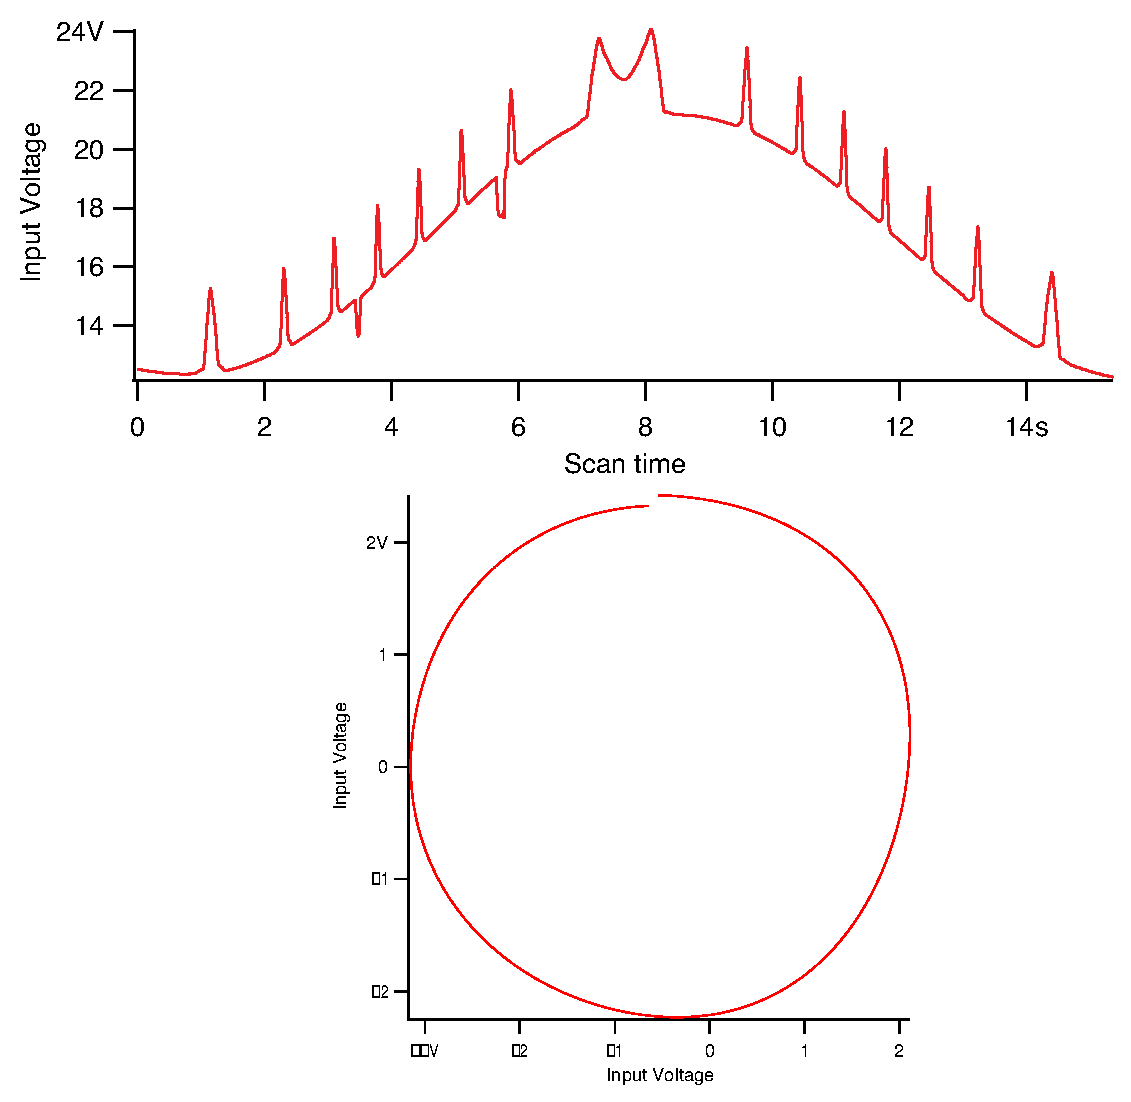
\includegraphics[scale=0.3]{images/tiltcircles.eps}
    \caption{Output of the tilt pattern}
  \label{tiltcircle}
\end{figure}

Then we compute our fitting algorithm on the x,y and z data.
\begin{table}[H]
\caption{Planefit coefficients} % title of Table
\centering % used for centering table
\begin{tabular}{c c c} % centered columns (4 columns)
\hline\hline %inserts double horizontal lines
$a_1$ & $a_2$ & $a_3$ \\ [0.5ex] % inserts table 
%heading
\hline % inserts single horizontal line
-0.14615  & -0.031882 & 29.537 \\[1ex]

\hline %inserts single line
\end{tabular}
\label{table:planefit} % is used to refer this table in the text
\end{table}

The size of the scan is still 30 um and the spiral has 80 loops. The scan pattern we are going to send to the controller is generated with the previously computed planefit coefficients. 

\begin{figure}[H]
  \centering
  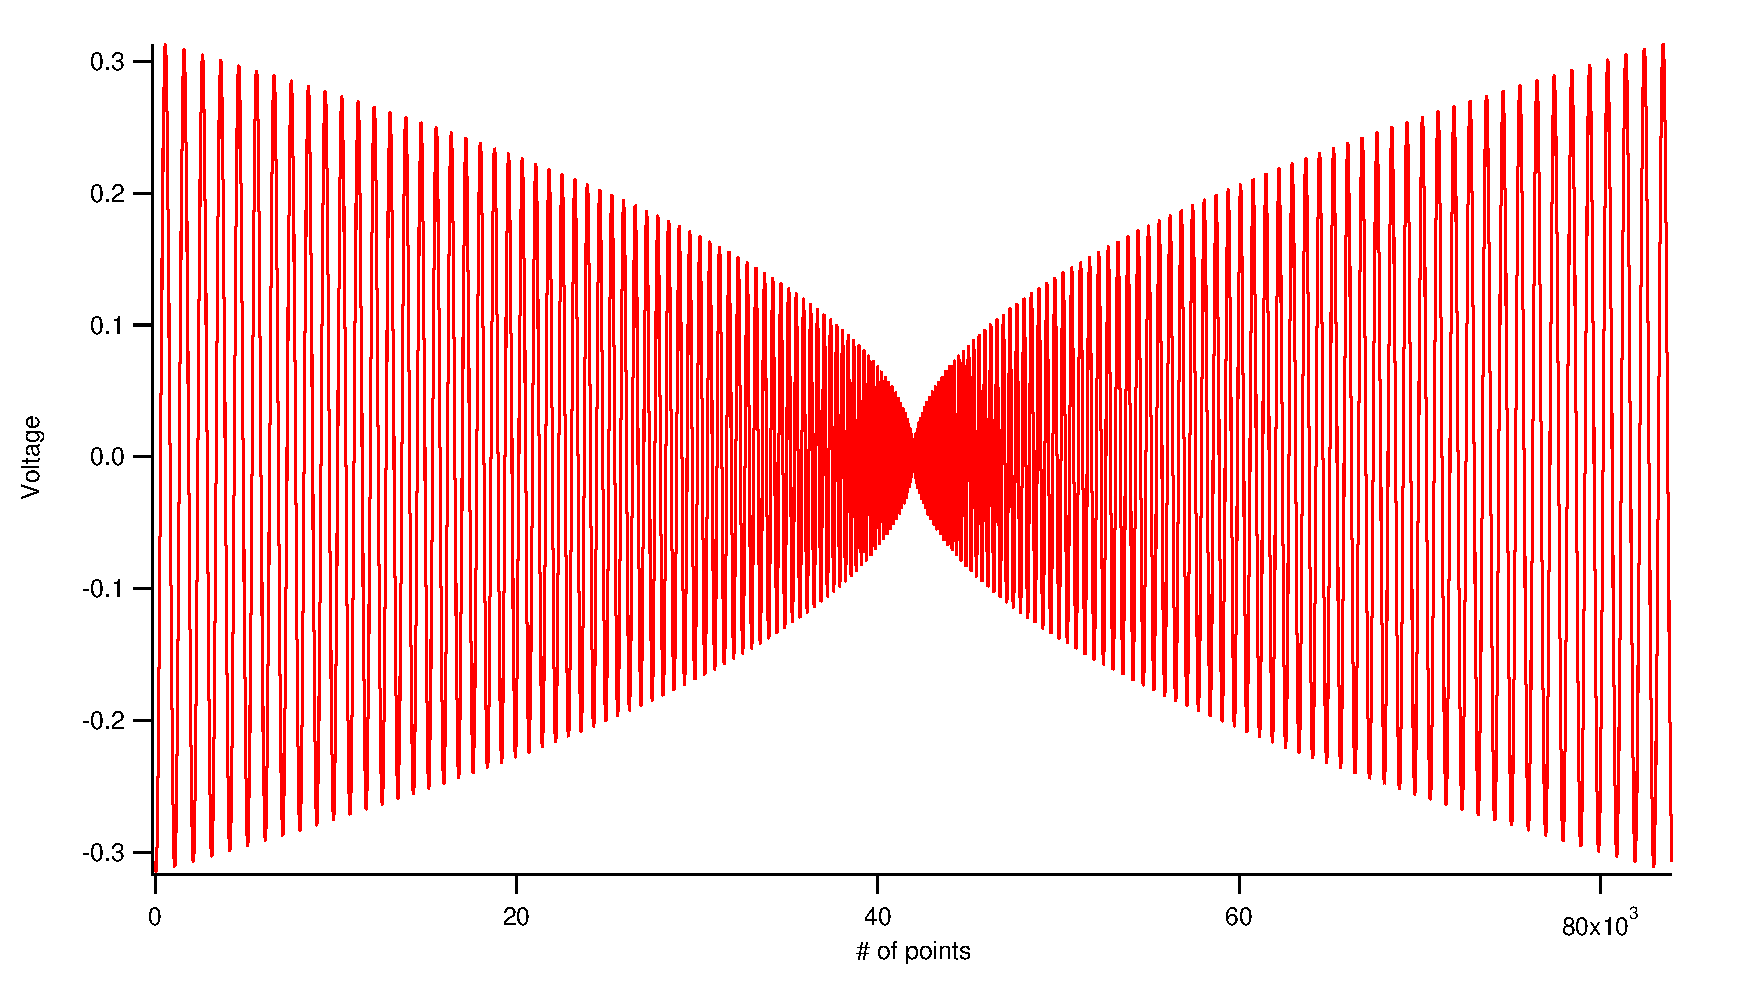
\includegraphics[scale=0.1]{images/spiralztiltout.eps}
    \caption{Input of the tilt compensation}
  \label{spiralztiltout}
\end{figure}



\begin{figure}[H]
  \centering
  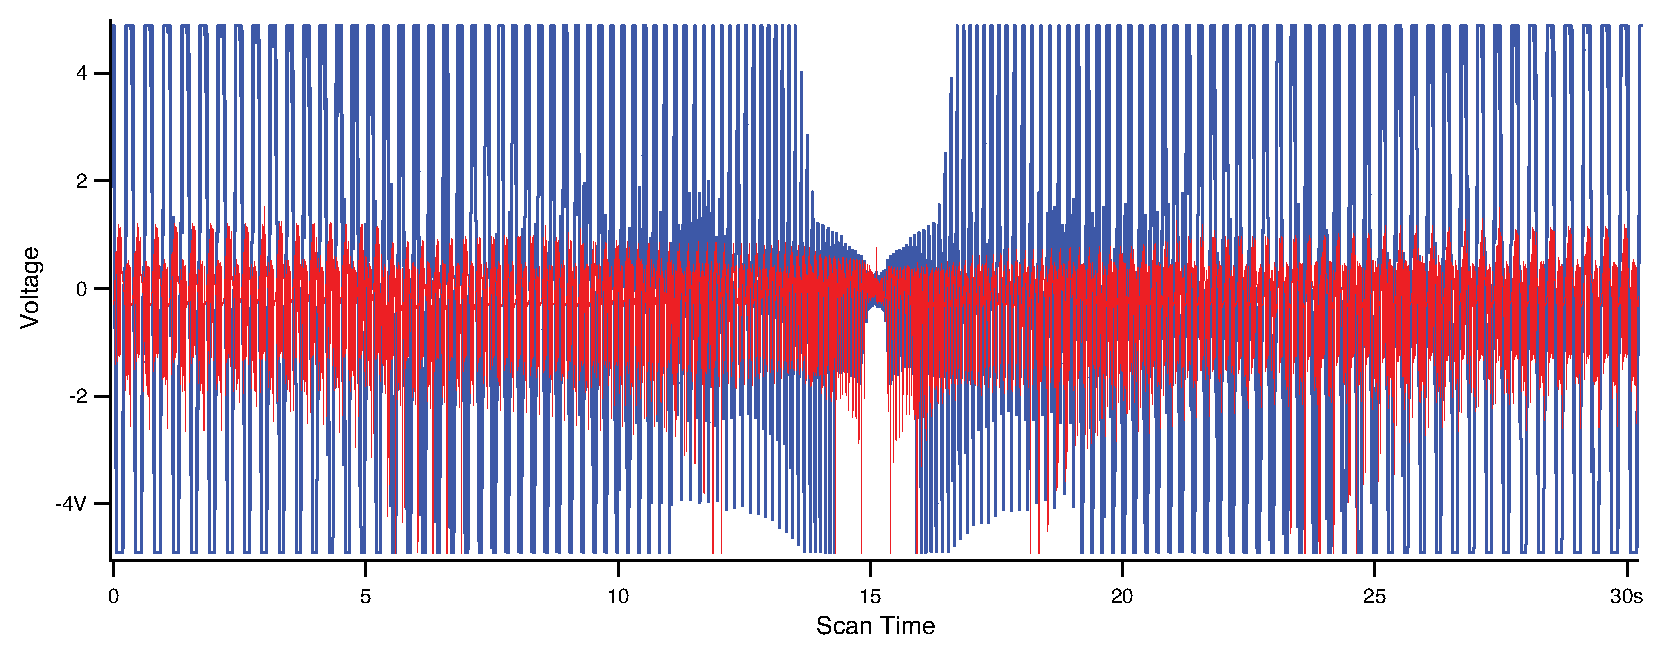
\includegraphics[scale=0.1]{images/tiltcorrectiongraph.eps}
    \caption{Output of the fast piezo}
  \label{spiralzfast}
\end{figure}


The tilt compensation will take a load off the small fast piezoelectrical ceramics. The Figure ~\ref{spiralzfast} shows the efficiency of our method. Indeed, the fast piezo was previously saturating. The piezos was trying to reach features that are larger than his range. If we use the tilt correction, we see that our piezo has no problem reaching those features.
